\begin{figure*}[t]
\fourColsNoDivide{0.22}{.18}{.275}{.25}
{
  \raisebox{-5pt}{\experimentv{$\Exp{\errep}_{\struct,\delta,r}(\advA)$
          \diffminus{$\Exp{\erreps}_{\struct,\delta,r}(\advA)$}}}\\[2pt]
    $\setP \gets \emptyset$; $\ct \gets 0$; $\key \getsr \keys$\\
    $i \getsr \advA^{\REPO,\UPO,\QRYO,\highlighto{\REVO}}$\\
    \diffminus{if $i \in \setP$ then return 0} \\[2.0pt]
    return $[\sum_\qry \err_i[\qry] \geq r]$
  \\[8pt]
  \diffplusbox{
  \oraclev{$\HASHO(X)$}\\[2pt]
    if $X \not\in \setX$ then return $\bot$\\
    if $T[X]=\bot$ then $T[X] \getsr \setY$\\
    return $T[X]$
  }\vspace{-4pt}
}
{
  \oraclev{$\REPO(\col)$}\\[2pt]
    $\pub \getsr \Rep_\key(\col)$\\
    if $\pub = \bot$ return $\bot$\\
    $\ct\gets\ct+1$ \\
    $\pub_\ct \gets \pub$\\
    %$\setC_\ct \gets \emptyset$\\
    $\col_\ct \gets \col$\\
    $\mathsf{rv} \gets \pub_\ct$; \diffminus{$\mathsf{rv} \gets \top$}\\
    return $\mathsf{rv}$
}
{
  \oraclev{$\UPO(i, \up)$}\\[2pt]
    %$X \gets \col^{v[i]}_i
    %$v[i] \gets v[i]+1$\\
    $\pub \getsr \Up_\key(\pub_i, \up)$\\
    if $\pub = \bot$ return $\bot$\\
    $\col_i \gets \up(\col_i)$\\
    $\pub_i \gets \pub$\\
    for $\qry$ in $\err_i$ do\\
    \tab $a \gets \Qry_K(\pub_i, \qry)$\\
    \tab if $\err_i[\qry] > \delta(a,\qry(\col_i))$ then\\
    \tab\tab$\err_i[\qry] \gets \delta(a,\qry(\col_i))$\\
    $\mathsf{rv} \gets \pub_i$; \diffminus{$\mathsf{rv} \gets \top$}\\
    return $\mathsf{rv}$
}
{
  \oraclev{$\QRYO(i, \qry)$}\\[2pt]
    $a \gets \Qry_K(\pub_i, \qry)$\\
    if $\err_i[\qry] < \delta(a,\qry(\col_i))$ then\\
    \tab$\err_i[\qry] \gets \delta(a,\qry(\col_i))$\\
    return $a$
  \\[6pt]
  \oraclev{$\REVO(i)$}\\[2pt]
    $\setP \gets \setP \cup \{i\}$ \\
    return $\pub_i$
}
  \caption{Two notions of adversarial correctness. The \errep\ notion captures
  correctness when the representation is always known to the adversary, while
  the \erreps\ notion captures correctness when the representation is secret.
  When modeling a function $H:\setX\to\setY$ as a random oracle, the $\HASHO$
  oracle is given to $\advA$, $\Rep$, $\Up$ and $\Qry$.}
  \vspace{6pt}\hrule
  \label{fig:security}
\end{figure*}


\newcommand{\oneColCCS}[2]{
  \makebox[.3\textwidth]{
    \begin{tabular}{|@{\gamespadleft}l@{\gamespad}|}
    \hline
    \rule{0pt}{1\normalbaselineskip}
    \begin{minipage}[t]{#1\textwidth}\gamesfontsize
      #2 \vspace{6pt}
    \end{minipage} \\
    \hline
  \end{tabular}
  }
}

\ignore{
\begin{figure}[t]
\oneColCCS{0.25}
{
\oraclev{$H(X)$}\\[2pt]
$V \getsr \mathcal{V}$\\
if $\mathrm{T}[X] \neq \undefn$ then $V \gets \mathrm{T}[X]$\\
$\mathrm{T}[X]\gets V$\\
return~$V$
}
\caption{Pseudocode for a Random Oracle~$H$ with outputs in set $\mathcal{V}$}
\label{fig:ROM}
\end{figure}
}

We define two adversarial notions of correctness given by a pair of related experiments for a mutable data structure $\struct$ and error capacity $r$, one in which the representations of the true data are public ($\errep$), and one in which they are private ($\erreps$).  We will describe the former, as the latter is a closely related derivative.  Throughout, we assume that the adversary~$\advA$ does not make any pointless queries. 

While many potential errors may exist for a given representation of a set, in the form of queries $\qry$ that would return an inaccurate answer when sent to $\QRYO$, we want an experiment that forces the adversary to actually find specific erroneous queries. In particular, we only give the adersary credit when they actually make a $\QRYO$ call that produces an error.

Both experiments aim to capture the total weight of the errors caused by the adversary, at any point in time, with respect to the current data objects $\col_i$ and their representations $\pub_i$.  Because we consider mutable data objects and representations, the notion of ``current'' is defined by calls to the $\REPO$ and $\UPO$ oracles.  Specifically, for each~$\col_i$, both experiments maintain a set~$\setC_i$ that is initially set to empty (when~$\col_i$ is first assigned via a~$\REPO$-query), and it is reset to empty whenever~$\col_i$ is updated via an $\UPO$-query.  This is capturing the fact that applying a non-empty update function~$\up$ to~$\col_i$ produces a new data object.

To track errors, both experiments maintain an array $\err_i[]$ for every data object~$\col_i$ that has been defined.   Initially, $\err_i[]$ is implicitly assigned the value of~$\undef$ at every index.  For purposes of value comparison, we adopt the convention that $\undef < n$ for all $n \in \mathbb{R}$.
%
Now, the array~$\err_i$ is indexed by query functions~$\qry$, and the value of $\err_i[\qry]$ is the ``weight'' of the error caused by~$\qry$, with respect to the \emph{current} data object~$\col_i$ and \emph{current} representation~$\pub_i$ (of~$\col_i$).  
%
The value of~$\err_i[\qry]$ is updated within the $\QRYO$- and $\UPO$-oracles, but observe that $\err_i[\qry] = \undef$ until $(i,\qry)$ is queried to the $\QRYO$-oracle.  Intuitively, a representation~$\pub_i$ of data object~$\col_i$ cannot surface errors until it is queried.

When~$\QRYO(i,\qry)$ executes, the value in $\err_i[\qry]$ is overwritten iff the error caused by~$\qry$ is larger than the existing value of $\err_i[\qry]$.  The first time $(i,\qry)$ is queried to~$\QRYO$ this is guaranteed, since the minimum possible value of $d$ is 0.  Since the set $\setC_i$ is used to prevent (WLOG) the adversary from repeating a query~$\QRYO(i,\qry)$ for a given~$\col_i$, increases to the value of $\err_i[\qry]$ may only be made ``across'' updates to~$\col_i$.  This may seem to be overly conservative, as an error-heavy~$\col_i$ may become less so after an update.  But we account for this within the $\UPO$-oracle.
In particular, calls to the $\UPO$-oracle may only \emph{decrease} the value of~$\err_i[\qry]$.  

When a query $\UPO(i,\up)$ is made, the oracle first updates the data object~$\col_i$ and its corresponding representation.  The set~$\setC_i$ is reset to empty, because the data object~$\col_i$ is ``new'' again.
%
Now, for each defined value~$\err_i[\qry]$, we reevaluate the error that \emph{would} be caused by the previously asked~$\qry$ w.r.t. the newly updated $\col_i$ and $\pub_i$.  If the existing value of $\err_i[\qry]$ is larger than the error that~$\qry$ would cause to w.r.t. the newly updated~$\col_i$ and $\pub_i$, then we overwrite $\err_i[\qry]$ with the smaller value.  Doing so insures that the array~$\err_i$ does not overcredit the attacker for errors against the current data object and representation.

For a concrete example of why these choices are necessary, consider a representation~$\pub$ of the set~$\col = \{1,2,3\}$ in some structure that supports set membership queries. Suppose an adversary learns that~$4$ is a false-positive value for $\pub$. If the adversary later uses an $\UPO$ query to add~$4$ to~$\col$, this should no longer count as a false positive. Our definition ensures that these known false positives are checked for and no longer counted if added to the set.

Given the experiments defined here, we define the advantage of an adversary $\advA$ as the probability it succeeds at the experiment, i.e. $\Adv{\errep}_{\struct,r}(\advA) = \Prob{\Exp{\errep}_{\struct,r}(\advA) = 1}$ in the public-representation case and $\Adv{\erreps}_{\struct,r}(\advA) = \Prob{\Exp{\erreps}_{\struct,r}(\advA) = 1}$ in the private-representation case. For constants $t$, $q_R$, $q_T$, $q_U$, $q_H$, we define $\Adv{\errep}_{\struct,r}(t,q_R,q_T,q_U,q_H)$ to be the maximum advantage attained by an adversary running in $t$ time steps and making $q_R$ calls to $\REPO$, $q_T$ calls to $\QRYO$, $q_U$ calls to $\UPO$, and $q_H$ calls to a random oracle. The advantage is defined analagously in the private-representation setting.

%%%%%%%%%%%%%%%%%%%%%%%%%%%%%%%%%%%%%%%%%%%%%%%%
\subsection{Generic results}
First, we note that any structure which is insecure in the immutable case is also insecure in the mutable case. Any adversary in the immutable case is identical to a corresponding adversary in the mutable case which simply never makes use of the $\UPO$ oracle. From this we know that standard (unsalted, unkeyed) Bloom filters cannot ensure correctness in the mutable case. 


\heading{Keyless structures.}

In a keyless structure, we assume all details of the algorithm used are known beforehand by the adversary, except any which might be generated `on the fly' as representations are created and modified. For example, many of these structures will assume the use of a random salt which is picked at the time the representation is created. A structure with neither randomization nor a private key is usually vulnerable to pre-computation and offline attacks, where the adversary can search for errors to produce without having to interact with the structure itself.

In many cases, it is easier to reason about an adversary which only has the chance to create and manipulate a single representation, rather than being able to call a $\REPO$ oracle as many times as it likes. Fortunately, in the case of keyless structures we can show that the adversary's advantage in a single-representation case is bounded above by a multiple of the advantage in the general case. We use $\errep1$ and $\erreps1$ to denote the public-representation and private-representation experiments where the adversary makes a single $\REPO$ query. In writing the advantage for these games we omit the $q_R$ parameter since it is fixed at 1.

%There are two equivalent ways of defining the $\errep1$ experiment. First, we may define it as a modified version of $\errep$ in which the adversary is constrained to make no more than one call to $\REPO$. We may equivalently define it as a two-stage adversary in the experiment below.

%\begin{figure}[t]
  \twoColsNoDivide{0.48}
  {
     \raisebox{-5pt}{\experimentv{$\Exp{\errep1}_{\struct,r}(\advA)$ {\colorbox{lightgray}{$\Exp{\erreps1}_{\struct,r}(\advA)$}}}}\\[2pt]
      $\setP \gets \emptyset$\\
      $\key \getsr \keys$\\
      $\col \getsr \advA$\\
      $i \getsr \advA^{\UPO,\QRYO}(\REPO(\col))$\\
      return $[\sum_\qry \err[\qry] \geq r]$ 
    \\[6pt]
    \oraclev{$\REPO(\col)$}\\[2pt]
      $\pub \getsr \Rep_\key(\col)$\\
      $\setC \gets \emptyset$\\
      $\mathrm{rv} \gets \pub$ \highlight{;\mathrm{rv} \gets \top} \\
      return $\mathrm{rv}$
  }
  {
    \oraclev{$\UPO(\up)$}\\[2pt]
%      $X \gets \col^{v[i]}_i
%      $v[i] \gets v[i]+1$\\
      $X \gets \col$ \\
      $\col \gets \up(X)$\\
      $\pub \getsr \Up_\key(\pub, \up)$\\
      $\setC \gets \emptyset$\\
      for $\qry$ in $\err$ do\\
      \tab $a \gets \Qry_K(\pub, \qry)$\\
      \tab if $\err[\qry] > d(a,\qry(\col))$ then\\
      \tab\tab$\err[\qry] \gets d(a,\qry(\col))$\\
      $\mathrm{rv} \gets \pub$ \highlight{;\mathrm{rv} \gets \top}\\
      return $\mathrm{rv}$
      \medskip

    \oraclev{$\QRYO(\qry)$}\\[2pt]
      if $\qry \in \setC$ then return $\bot$\\
      $\setC \gets \setC \union \{\qry\}$\\
      $a \gets \Qry_K(\pub, \qry)$\\
      if $\err[\qry] < d(a,\qry(\col))$ then\\
      \tab$\err[\qry] \gets d(a,\qry(\col))$\\
      return $a$
  }
  \caption{The $\errep1$ adn $\erreps1$ notions of adversarial correctness. These are equivalent to the standard $\errep$ and $\erreps$ notions where the adversary is only allowed to make a single call to $\REPO$.}
  \vspace{6pt}\hrule
  \label{fig:security}
\end{figure}

Note that in the $\erreps1$ scenario we need not provide the adversary with a $\REVO$ oracle. If the adversary uses only a single representation, may assume without loss of generality that they make no call to $\REVO$, since doing so would prevent the adversary from having any possibility of winning. Since the case of a single $\REPO$ query is considerably simpler to handle, the first step in each of our proofs will be to reduce $\errep$ and $\erreps$ to $\errep1$ and $\erreps1$ respectively. In addition to this, we wish to move from actual hash functions to true random functions. Using the following lemmas, we may reduce the case of $\errep$ for any structure using a salted hash to the case of $\errep1$ using a true random function, and we may reduce $\erreps$ for a structure using a secret-keyed hash to the case of $\erreps1$ using a true random function.

\begin{lemma}[\errep1 and \erreps1 imply \errep and \erreps for keyless structures]\label{lemma:errep}
  Let $\struct = (\Rep, \Qry, \Up)$ be a data structure with key
  space $\{\emptystr\}$. For every $t, q_R, q_T, q_U, q_H, r\geq 0$, it holds that
  \[
    \Adv{\errep}_{\struct,r}(t, q_R, q_T, q_U, q_H) \leq
    q_R\cdot\Adv{\errep1}_{\struct,r}(O(f(t)), q_T, q_U, q_H) \,,
  \]
  where $f(t) = t + (q_R-1)\ticks(\Rep,t) + q_T\ticks(\Qry,t) + q_U\ticks(\Up,t)$.
\end{lemma}

\begin{proof}For a fixed $r \ge 0$, let $\advA$ be an $\errep$ or $\erreps$ adversary which runs in $t$ time steps and makes $q_R$ $\REPO$ queries, $q_T$ $\QRYO$ queries, $q_U$ $\UPO$ queries, and $q_H$ RO queries. We construct an adversary $B$ for $\errep1$ or $\erreps1$, respectively, as follows.

First, $\advB$ initializes a counter $ct \gets 0$ and a set $\setC \gets \emptyset$, and samples $q \getsr [q_R]$. Next $\advB$ executes $\advA$, simulating the answers to its oracle queries as follows. When $\advA$ asks the query $\REPO(\col)$, $\advB$ sets $ct \gets ct + 1$ and stores $\col_{ct} \gets \col$. Then, if $ct = q$, $B$ forwards $\col$ to its own $\REPO$ oracle, returning the resulting value ($\pub$ in the public-representation case, or $\top$ in the private-representation case) to $\advA$. Otherwise, $\advB$ computes $\pub_{ct} \getsr \Rep(\col)$ and returns either $\pub_{ct}$ or $\top$. When $\advA$ asks for the query $\QRYO(i,\qry)$, $\advB$ first checks if $(i,\qry) \in \setC$ and returns $\bot$ if this condition holds. Otherwise $\advB$ forwards $(i,\qry)$ to its $\QRYO$ oracle and returns $a$ if $i = q$, and reutrns $\Qry(\pub_i,\qry)$ otherwise. Similarly, when $\advA$ makes an $\UPO(i,\up)$ query, $\advB$ forwards $(i,\up)$ to its $\UPO$ oracle if $i = q$ and evaluates $\Up(\pub_i,\up)$ otherwise. Finally, queries from $\advA$ to its RO are simply forwarded to $\advB$'s RO. When $\advA$ halts and outputs $j$, $\advB$ does the same.

If $j = q$, then $B$ wins if $A$ does, since all queries from $A$ to $\pub_j$ were forwarded to $B$'s $\QRYO$ oracle. Given that $q$ is sampled uniformly from the range $[q_R]$, it follows that

$$\Adv{\errep}_{\struct,r}(t, q_R, q_T, q_U, q_H) \leq q_R\cdot\Adv{\errep1}_{\struct,r}(O(f(t)), q_T, q_H).$$

Note that $B$ makes at most $q_T$ queries to $\QRYO$ and $q_H$ queries to its RO. Since $A$ runs in $t$ time steps and writing a bit takes 1 time step, the input length to any $\Rep$, $\Qry$, or $\Up$ evaluated by $B$ is at most $t$ bits. Hence, adversary $B$ runs in time $O(t+(q_R-1)\ticks(\Rep,t)+q_T\ticks(\Qry,t)+q_U\ticks(\Up,t))$.\missingqed
\end{proof}

\begin{lemma}[In the ROM, salted hashing is almost as good as distinct random functions in \errep1]\label{lemma:salttorand}
  Let $\struct = (\Rep, \Qry, \Up)$ be a data structure with key space $\{\emptystr\}$ and salt space $\bits^\lambda$, and let $\struct'$ be the same structure using true random functions in place of salted hash functions. For every $t, q_R, q_T, q_U, q_H, r \geq 0$, it holds that
  \[
    \Adv{\errep1}_{\struct,r}(t, q_R, q_T, q_U, q_H) \leq \frac{q_H}{2^\lambda} + \Adv{\errep1}_{\struct',r}(t, q_R, q_T, q_U, q_H)
  \]
\end{lemma}

\begin{proof}
Let $\G_0$ be the standard $\errep1$ game for the structure $\struct$, and let $\G_1$ be the same game for $\struct'$. There exists an adversary $\advB$ such that $\Prob{\G_0(\advA) = 1} \le \Prob{\G_1(\advB) = 1} + q_H/2^\lambda$. This adversary initializes an empty table $R$ and simulates $\advA$. When a query $w$ is sent to $\HASHO$, $\advB$ returns $R[w]$ if this entry in the table is defined. Otherwise, if $w = \langle\salt, x\rangle$ for some $\salt \in \bits^\lambda$ and $x \in \bits^*$, forward $(\salt, x)$ to $\HASHO$, store the result in $R[w]$, and return this value. Finally, if $R[w]$ is not defined and $w$ is not of this form, sample $r$ uniformly from the range of the hash function, store the result in $R[w]$ and return that result. Queries to all other oracles are simply forwarded to $\advB$'s oracle. Assuming the output of the hash function is uniformly distributed, this simulation is perfect unless $\advA$ guesses the salt correctly, which happens with probability $q_H/2^\lambda$.\missingqed
\end{proof}

\heading{Keyed structures.}

As in the keyless case, we can reduce the case of $\erreps$ for a secretly-keyed hash to the case of $\erreps1$ using a true random function. Though the proof is different, we achieve a similar bound as in the unkeyed private-representation case. Despite the similar-looking bounds, the secret-keyed case is preferable in practice because the $q_R$ $\REPO$ queries are `online' while the $q_H$ $\HASHO$ queries are `offline', limited only by the computational capabilities of the adversary.

\begin{lemma}[\errep1 with random functions implies \errep with keyed hashing]\label{lemma:keytorand}
  Let $\struct = (\Rep, \Qry, \Up)$ be a data structure with key space $\mathcal{K}$ and salt space $\bits^\lambda$, and let $\struct'$ be the same structure using true random functions in place of salted and keyed hash functions. For every $t, q_R, q_T, q_U, q_H, r \geq 0$, it holds that
  \[
    \Adv{\errep1}_{\struct,r}(t, q_R, q_T, q_U, q_H) \leq \frac{q_R^2}{2^\lambda} + q_R \cdot \Adv{\errep1}_{\struct',r}(t, q_R, q_T, q_U, q_H)
  \]
\end{lemma}

\begin{proof}
In each of the structures considered here, we model the use of a secretly keyed hash function with the use of a pseudorandom function $F_K$. Let $\G_0$ be the $\errep$ game on this structure. Our first step is to move to a game $\G_1$ where the pseudorandom function $F_K$ is replaced by a true random function $\Rnd$ which is lazily evaluated as necessary when $\REPO$, $\QRYO$, and $\UPO$ are called. By a conditioning argument, the advantage of the adversary is given by $\Adv{\errep}_{\struct,r}(\advA) = \Adv{\prf}_F(\advB) + \Prob{\G_1(\advA)=1}$.

Consider another game $\G_2$ that ensures the salts do not repeat, by choosing $\salt$ exclusively from salts which have not been previously used. The game is identical to $\G_1$ until a salt repeats, which by the birthday bound occurs with probability $q_R^2/2^\lambda$. Therefore $\Adv{\errep}_{\struct,r}(\advA) = \Adv{\prf}_F(\advB) + q_R^2/2^\lambda + \Prob{\G_2(A) = 1}$.

Next, we revise the game to $\G_3$ where the adversary gets credit for queries $\QRYO(i,\qry)$ which are false positives for any $\pub_j$, regardless of the actual argument $i$ given to $\QRYO$. Since this can only benefit the adversary, $\Adv{\errep}_{\struct,r}(\advA) \le \Adv{\prf}_F(\advB) + q_R^2/2^\lambda + \Prob{\G_3(A) = 1}$.

However, because each representation makes use of a random function for determining the value of all representations, updates, and queries, the probability of a previously unqueried element producing an error in one representation is independent of its probability of producing an error in the other representations. When we move to the final game $\G_4$ where the adversary is only allowed to call $\REPO$ once, the adversary's advantage will then decrease by a factor of at most $q_R$. This gives us the final result:

$$\Adv{\errep}_{\struct,r}(\advA) \le \Adv{\prf}_F(\advB) + \frac{q_R^2}{2^\lambda} + q_R \cdot \Prob{\G_4(A) = 1}$$\missingqed
\end{proof}

\heading{Invertible structures.}

Several structures are designed to implement both insertion and deletion operates. This allows the adversary a great deal of variety in the updates it can perform during the security experiment. For a more general notion, we define an \textit{invertible} structure as one where, for any initial representation $\pub$ and any other representation $\pub' = \Up_K(\ldots\Up_K(\pub,\up_1)\ldots,\up_n)$ generated by a sequence of update operations applied to the initial representation, there exists another sequence of update operations such that $\Up_K(\ldots\Up_K(\pub',\up'_1)\ldots,\up'_m) = \pub$. In other words, any sequence of updates applied to any representation can be undone by further updates.

\begin{lemma}[Salts do not affect \errep for invertible structures]\label{lemma:noinvsalt}
  Let $\struct = (\Rep, \Qry, \Up)$ be a data structure with a salt randomly initialized at runtime and $\struct'$ be the same structure using a fixed value from the salt space in place of a randomized salt. For every $t, q_R, q_T, q_U, q_H, r\geq 0$, it holds that
  \[
    \Adv{\errep}_{\struct,r}(t, q_R, q_T, q_U, q_H) \leq
    \Adv{\errep}_{\struct',r}(O(t), 1, q_T, q_U+2n(q_R+q_T+q_U), q_H) \,,
  \]
  where $n$ is the longest minimal sequence of update operations needed to generate a data structure in the space.
\end{lemma}
\begin{proof}
Consider an adversary $A$ in the case of a non-salted data structure which makes $q_R$ queries to $\REPO$ and $q_T$ queries to $\QRYO$. We construct an adversary $B$ for the salted case which produces the same errors as follows. First, $B$ initializes a counter $ct$ to 0 and calls the $\REPO$ oracle on the empty set, receiving an empty representation $\pub$ together with the salt used to create the representation. Then $B$ runs $A$, answering its oracle queries as follows. Whenever $A$ makes a query of the form $\REPO(\col)$, $B$ sets $ct \gets ct + 1$ and calls $\UPO$ repeatedly on $\pub$ to transform it into a representation of $\col$. Then $B$ returns the modified $\pub$ to $A$, stores $\col_{ct} \gets \col$, and performs the opposite updates in reverse order to return to the original empty representation $\pub$. If $A$ makes a query of the form $\QRYO(i,\qry)$, $B$ calls $\UPO$ repeatedly to transform $\pub$ into a representation of $\col_i$ and then returns the result of querying its own oracle with $\QRYO(1, \qry)$. Then once again $B$ performs the inverse updates to transform $\pub$ back into the original empty representation. If $A$ queries for $\UPO(i, \up)$, $B$ sets $\col_i \gets \up(\col_i)$ and again uses $\UPO$ queries to transform $\pub$ into a representation of $\col_i$, returns the value of $\pub$, and then performs opposite $\UPO$ queries to return $\pub$ to the empty representation. Finally, $B$ forwards any of $A$'s RO queries to its own RO.

In general this may use as many as $2n(q_R+q_T+q_U)$ update queries, where $n$ is the longest minimal sequence of update operations needed to generate a data structure in the space. Furthermore $B$ succeeds if $A$ does, so the adversaries' advantages are equal.\missingqed
\end{proof}

%\subsection{Immutabilization}

%We say that a structure has `independent representations' if knowing the representation of one set does not provide any additional information about the representation of any other set. More formally, $\Pi$ has independent representations if $\Prob{\Rep_K(\col) = \pub | \Rep_K(\col')}$

%For example, the standard Bloom filter vacuously has independent representations, since the adversary can perfectly predict the representation of any set without needing to see the representation of other sets. A filter which uses true random sampling in place of hash functions also has independent representations, but a filter which uses a secret key need not have independent representations.

%In each of our example structures involving the use of a secret key, we formalize the system using a pseudorandom function. In each correctness proof, the first thing we do is always moving to a game where the pseudorandom functions are replaced by true random functions, since this gives very similar adversarial advantage (assuming the use of a good prf) while making the behavior of the game much easier to reason about.

%In the case of a structure with sufficiently `independent' representations, we may assume without loss of generality that the adversary never calls the $\REVO$ oracle, since doing so can only decrease their probability of success.

%Note that most of the data structures we consider have some degree of per-representation randomness, such as a salt chosen for hash functions. We consider an alternate correctness game that forces this randomness to behave the same across all representations constructed. In particular, any randomly-chosen parameters which would be chosen during the computation of $\REPO$ are selected at the beginning of the game, using the same random distribution, before the adversary makes any oracle queries. The $\REPO$ oracle then uses this fixed value for any random parameters in place of sampling a new random value.

%\begin{lemma}[]\label{lemma:immutabletomutable}
%  Let $\struct = (\Rep, \Qry, \Up)$ be a data structure, and $\struct'$ be the same structure except that any per-representation random parameters are chosen once and fixed across representations. For every $t, q_r, q_T, q_U, q_H, q_V, r \geq 0$, it holds that
%  \[
%    \Adv{\errep}_{\struct,r}(t, q_R, q_T, q_U, q_H, q_V) \leq
%    \Adv{\prf}_F(\advB) + \Adv{\errep}_{\struct',r}(O(t), q_R + q_U, q_T, 0, q_H, 0) \,,
%  \]
%\end{lemma}
%\begin{proof}
%Given an adversary $\advA$ making queries $(q_R, q_U, q_T, q_H)$, we can construct $\advB$ making queries $(q_R+q_U, 0, q_T, q_H)$ which achieves the same advantage.

%For a structure $\Pi$, we denote by $\Pi'$ the same structure with pseudo-random functions replaced by true-random functions. Using conditional probabilities, we have $\Adv{\errep}_{\struct,r}(\advA) \le \Adv{\prf}_F(\advB) + \Adv{\errep}_{\struct_1,r}(\advA)$.

%In the truly random structure $\struct_1$, the representation of a set is simply a randomly-chosen valid representation of that set. Revealing this therefore reveals no new information about any other representations which have been constructed, and so calling $\REVO$ can only decrease an adversary's chance of success. We may now assume $\REVO$ is never called.

%We next modify the structure to $\struct_2$, where all randomized parameters are fixed across representations at the beginning of the experiment, but not revealed to the adversary. We create an adversary $C$ for the correctness experiment on $\struct_2$ which simulates $\advA$ as follows. The adversary $C$ keeps track of a counter $ct$ and list $L$ of indices and simulates $\advA$. When $\advA$ calls $\REPO$, $C$ appends $ct$ to the end of $L$ and then increments $ct$. When $\advA$ calls $\UPO(i,\up)$, $C$ calls $\REPO(\up(\col_{I(i)}))$, sets $L(i) \gets ct$, and increments $ct$. Finally, when $\advA$ calls $\QRYO(i,\qry)$, $C$ calls $\QRYO(L(i),\qry)$. Since $\REVO$ is never called, $C$ need not implement this oracle. Since all queries are called on representations of the same sets, $C$ has the same probability of success as $A$.
%\end{proof}

\subsection{Bloom filter results}
\label{subsec:bloom-filters}

%\subsection{Bloom filter lower bounds}

%\begin{table}[thp]
\begin{center}
  \begin{tabular}{ | c | c |c | c | c | }
    \hline
    Salt & Key & \parbox{.75in}{Private\\ Representation} & \parbox{.75in}{Irreversible\\ Updates} & Result \\ \hline\hline
    0 & 0 & 0 & 0 & Attack 1 \\ \hline
    0 & 0 & 0 & 1 & Attack 1 \\ \hline
    0 & 0 & 1 & 0 & Attack 1 \\ \hline
    0 & 0 & 1 & 1 & Attack 1 \\ \hline
    0 & 1 & 0 & 0 & Attack 2 \\ \hline
    0 & 1 & 0 & 1 & Attack 2 \\ \hline
    0 & 1 & 1 & 0 & Attack 2 \\ \hline
    0 & 1 & 1 & 1 & Attack 2 \\ \hline
    1 & 0 & 0 & 0 & Attack 3 \\ \hline
    1 & 0 & 0 & 1 & Attack 3 \\ \hline
    1 & 0 & 1 & 0 & ? \\ \hline
    1 & 0 & 1 & 1 & Theorem~\ref{thm:bf-priv-salt-bound} \\ \hline
    1 & 1 & 0 & 0 & Attack 4 \\ \hline
    1 & 1 & 0 & 1 & Theorem~\ref{thm:bf-key-bound} \\ \hline
    1 & 1 & 1 & 0 & ? \\ \hline
    1 & 1 & 1 & 1 & Theorem~\ref{thm:bf-key-bound} \\
    \hline
  \end{tabular}
\end{center}
\tsnote{This table feels unintutive, somehow. ``Salt'', ``Key'', ``Irreversible updates'' are all syntactic properties; ``Private Representation'' is an artifact of the attack model.  We need a better way to organize and present these results.}
\caption{Summary table for Bloom filters. \textbf{Attack 1:}The adversary chooses a maximally large test set $\col$ and simulates $\Rep$ to produce a representation $\pub$. The adversary then simulates $\Rep$ for many arbitrarily chosen singleton sets disjoint from $\col$, checking each one to see if its element is a false positive for $\pub$. Once it has accumulated $r$ false positives, call $\REPO$ on $\col$, call $\QRYO$ for each false positive found, and return 1.  \textbf{Attack 2:} The adversary chooses a maximally large test set $\col$ and calls $\REPO$ to produce a representation $\pub$. The adversary then calls $\REPO$ for many arbitrarily chosen singleton sets disjoint from $\col$, using $\QRYO$ on each to determine if its element is a false positive for the representation constructed for $\col$. Once it has accumualated $r$ false positives, return 1. \textbf{Attack 3:}  The adversary chooses a maximally large test set $\col$ and calls $\REPO$ to receive a representation $\pub$ together with the salt $\salt$. Using the known salt, the adversary simulates $\Rep$ for many arbitrarily chosen singleton sets disjoint from $\col$, checking each one to see if its element is a false positive for $\pub$. Once it has accumulated $r$ false positives, call $\QRYO$ for each such false positive and return 1. \textbf{Attack 4:}The adversary chooses a test set $\col_0$ and a target set $\col_1$, performing a search on representable subsets of $\col_0$ represented as a tree ordered by $\subseteq$. Moving up or down in the tree is accomplished using $\UPO$, and at each node $\QRYO$ is called for each element of $\col_1$ to determine which are false positives. Once $r$ false positives are found, halt and return 1. }
\label{tab:main}
\end{table}

The standard Bloom filter shows a variety of different behaviors depending on its exact implementation. If the hash functions used are chosen beforehand and potentially known to the adversary, this public information allows offline attacks to be mounted against the data structure which can produce potentially damaging false positives. In the case of immutable Bloom filters, making use of a per-representation salt is sufficient to prevent these attacks, though depending on the use case the use of non-fixed per-representation randomness may or may not be feasible. Furthermore, in the case of mutable Bloom filters there are additional difficulties with offline attacks due to adversarially-chosen updates. To guarantee correctness in this case we must additionally guarantee that representations can be kept private from the adversary.

A generic attack against unsalted, unkeyed data structures handling set membership queries is for the adversary to choose a large set $\col$ of potential filter elements and simulate $\REPO$ to produce representations for $\{x\}$ for each $x \in \col$. Given these, it can perform offline computations to determine disjoint $\setT$, $\setR \subseteq \col$ such that the elements of $\setR$ all produce errors when queried for membership in $\REPO(\setT)$. After a sufficiently large $\setR$ has been found, the adversary makes a single $\REPO$ call on $\setT$ and makes one $\QRYO$ call per element of $\setR$, resulting in guaranteed success for the adversary with only a minimal number of queries performed.

In general, such an attack may not be computationally feasible in the real world. However, because the attack is entirely offline, many structures with non-negligible error probabilities are vulnerable to these attacks. For example, consider a Bloom filter with false positive probability $10^{-5}$ with an adversary wishing to construct $r = 10$ false positives. The adversary can fix $\setT$ in advance and perform somewhere on the order of a million hash queries to random elements in order to construct a $\setR$ of size 10, and then perform only a single $\REPO$ calls and ten $\QRYO$ calls to the service hosting the Bloom filter. This is likely to be much more feasible for the adversary than performing on the order of a million $\QRYO$ calls in an online attack which randomly guesses elements until it accumulates 10 false positives.

The use of a salt without a private key in the public representation setting is insufficient to defeat this attack. In this setting, the adversary need only make its $\REPO$ query for $\setT$ in advance, at which point it will receive both the representation $\pub$ and the salt $\salt$ used to construct it. Using this known salt, the adversary is still able to simulate $\REPO$ for arbitrary singleton representations. The previous attack therefore still works with the same (minimal) number of $\QRYO$ calls at the very end of the experiment, after it has determined $\setR$ using offline computations.

The opposite of this, using a private key without a salt, does weaken the attack somewhat. Even with public representations, the adversary cannot locally simulate $\REPO$ without guessing the private key. However, they can still outperform random $\QRYO$ calls by making $\REPO$ queries for singleton elements without fixing any $\setT$ in advance. After selecting a random set $\col$ of size $q_R-1$, the adversary performs offline computations to find $\setT$, $\setR \subseteq \col$ such that the elements of $\setR$ are false positives for the representation of $\setT$ (which can be computed from the representations of the singleton subsets of $\setT$). The adversary wins if there is a partition where $\setR$ produces at least $r$ errors on $\REPO(\setT)$.

% ...

Using a salted Bloom filter in the private representation setting, however, does provide some security. At the time a representation is created, the structure chooses a salt $\salt$ which it will use for all further queries and updates. In order for maximum security to be guaranteed, we must ensure that the representation, and in particular the salt, is kept secret from the adversary. We define this structure $\SBF[H,k,m,n,\lambda]$ as the Bloom filter structure that uses $H(s) = (h_1(s),\ldots,h_k(s))$ for hashing inputs to $k$ values in $[m]$. Furthermore, each call of $\Rep$ first involves picking a salt $\salt$ from the salt space $\bits^\lambda$, and all hashes made to insert or query for an element $x$ are determined using $H(x \Vert \salt)$. Finally, the parameter $n$ means that any attempts to represent sets with more than $n$ elements fail.

\begin{theorem}[Correctness Bound for Private-Representation Salted Bloom Filters]\label{thm:bf-priv-salt-bound}
Fix integers $k, m, n, \lambda, r\geq 0$, let $H \colon \bits^* \to [m]$ be a function, and let $\struct_s = \SBF[H,k,m,n,\lambda]$.
  For every $t, q_R, q_T, q_H \geq 0$, it holds that
  \begin{eqnarray*}
    \Adv{\erreps}_{\struct_\saltybloom,r}(t,&q_R,& q_T, q_U, q_H) \leq \\ && q_R \cdot
     \left[
      \frac{q_H}{2^\lambda} +
      {\dbinom{q_T+q_U}{r}} p(k, m, n+r)^r
    \right] \,,
\end{eqnarray*}
where $H$ is modeled as a random oracle and $p(k, m, n+r)$ is the standard, non-adaptive false-positive probability on a Bloom filter with the given parameters.
\end{theorem}

This proof first reduces to the single-representation case, which as shown in lemma~\ref{lemma:errep} will reduce the adversary's advantage by at most a factor of $q_R$. The main idea behind the proof is to remove the adversary's adaptivity a step at a time. We isolate the possibility of the adversary guessing the salt, which would allow it to mount its own offline attack on the filter without relying on the $\QRYO$ oracle. If the adversary does not guess the salt, the outputs of the $\REPO$, $\QRYO$, and $\UPO$ oracles are unpredictable to the adversary, producing uniformly randomly distributed bits to set (for $\REPO$ and $\UPO$) or to check (for $\QRYO$). Under the assumption that the adversary does not predict the salt, queries made to distinct elements are independent of each other. The only remaining issue is that the adversary can potentially gain an advantage by testing whether some object $x$ is a false positive for the filter, and then updating the filter to include $x$ only if the test query returned `false'. An analysis shows that this is now (once imperfect pseudorandom functions and salt collisions have been dealt with) the only way for the adversary to gain an advantage over making queries to an immutable Bloom filter. Because this adaptive strategy introduces tricky conditional possibilities, we cannot compute an exact value for the adversary's advantage. Instead, we move to an alternate scenario where each $\QRYO$ also produces a free update and every $\UPO$ first performs a free query. This makes $\QRYO$ and $\UPO$ calls indistinguishable, so that the adversary is effectively making a series of independent random queries that each have a chance to increment the error counter. Because the number of 1s in the filter can only increase, the probability of a false positive from any one of these queries is bounded above by the probability of a false positive on the final maximally-sized filter, a probability which is given by the Kirsch and Mitzenmacher bound.

\begin{figure}
  \boxThmBFSaltCorrect{0.48}
  {
    \underline{$\G_0(\advA)$}\\[2pt]
      $\col \getsr \advA^H$; $\setC \gets \emptyset$; $\err \gets 0$\\
      $\pub \getsr \Rep[H](\col)$\\
      $\bot \getsr \advA^{H,\QRYO,\UPO}$\\
      return $(\err \geq r)$
    \\[6pt]
    \oraclev{$\QRYO(\qry_x)$}\\[2pt]
      if $\qry_x \in \mathcal{C}$ then return $\bot$\\
      $\setC \gets \setC \union \{\qry_x\}$\\
      $a \gets \Qry[H](\pub, \qry_x)$\\
      if $a \neq \qry_x(\col)$ then $\err \gets \err + 1$\\
      return~$a$
    \\[6pt]
    \oraclev{$\UPO(\up_x)$}\\[2pt]
      $\setC \gets \emptyset$\\
      $a \gets \Qry[H](\pub, \qry_x)$\\
      if $\qry_x \in \setC$ and $a \neq \qry_x(\col)$ then\\
      \tab $\err \gets \err-1$\\
      $\col \gets \col \union \{x\}$\\
      $\pub \gets \Up[H](\pub,\up_x)$\\
      return~$\bot$
    \\[4pt]
    \hspace*{-4pt}\rule{1.043\textwidth}{.4pt}
    \\[5pt]
    \oraclev{$\HASHO_1(\salt,x)$} \hfill\diffplus{$\G_2$}\;{$\G_1$}\hspace*{3pt}\\
      $\hh \getsr [m]^2$; $\vv \gets \fff(\hh$)\\
      if $\salt = \salt^*$ then\\
      \tab $\bad_1 \gets 1$; \diffplus{return $\vv$}\\
      if $T[\salt,x]$ is defined then $\vv \gets T[\salt,x]$\\
      $T[\salt,x] \gets \vv$;
      return $\vv$
  }
  {
    \underline{$\G_1(\advB)$}\\[2pt]
      $\salt^* \getsr \bits^\lambda$;
      $\col \getsr \advB^{\HASHO_1}$\\
      $\pub \gets \Repx[\HASHO_2](\col, \salt^*)$\\
      $\setC \gets \emptyset$;
      $\err \gets 0$\\
      $\bot \getsr \advB^{\HASHO_1,\QRYO,\UPO}$\\
      return $(\err \geq r)$
    \\[6pt]
    \oraclev{$\QRYO(\qry_x)$}\\[2pt]
      if $\qry_x \in \mathcal{C}$ then return $\bot$\\
      $\setC \gets \setC \cup \{\qry_x\}$\\
      $a \gets \Qry[\HASHO_2](\pub, \qry_x)$\\
      if $a \neq \qry_x(\col)$ then $\err \gets \err + 1$\\
      return~$a$
    \\[6pt]
    \oraclev{$\UPO(\up_x)$}\\[2pt]
      $\setC \gets \emptyset$\\
      $a \gets \Qry[H](\pub, \qry_x)$\\
      if $a \neq \qry_x(\col)$ and $\qry_x \in \setC$ then\\
      \tab $\err \gets \err-1$\\
      $\col \gets \col \union \{x\}$\\
      $\pub \gets \Up[\HASHO_2](\pub,\up_x)$\\
      return~$\bot$
    \\[6pt]
    \oraclev{$\HASHO_2(\salt,x)$}\\[2pt]
      $\hh \getsr [m]^2$; $\vv \gets \fff(\hh$)\\
      if $T[\salt,x]$ is defined then\\
      \tab $\vv \gets T[\salt,x]$\\
      $T[\salt,x] \gets \vv$;
      return $\vv$
  }
  {
    \underline{$\G_3(\advB)$}\\[2pt]
    \oraclev{$\QRYO(\qry_x)$}\\[2pt]
      $a \gets \Qry[\HASHO_3](\pub, \qry_x)$\\
      if $a \neq \qry_x(\col)$ then $\err \gets \err + 1$\\
      $\col \gets \col \union \{x\}$
      $\pub \gets \Up[\HASHO_2](\pub,\up_x)$\\
      return~$a$
  }
  {
    \oraclev{$\UPO(\up_x)$}\\[2pt]
      $a \gets \Qry[\HASHO_3](\pub, \qry_x)$\\
      if $a \neq \qry_x(\col)$ then $\err \gets \err + 1$\\
      $\col \gets \col \union \{x\}$
      $\pub \gets \Up[\HASHO_2](\pub,\up_x)$\\
      return~$\bot$
    \\[6pt]
    \oraclev{$\HASHO_i(\salt,x)$}\\[2pt]
      $\hh \getsr [m]^2$; $\vv \gets \fff(\hh$)\\
      return $\vv$
  }
  \caption{Games 0--3 for proof of Theorem~\ref{thm:bf-priv-salt-bound}.}
  \label{fig:bf-priv-salt-bound}
\end{figure}

\begin{proof} We first reduce from the $\erreps$ case to the $\erreps1$ case, which by lemma~\ref{lemma:errep} may scale the adversary's advantage only by a factor of $q_R$. The game~$\G_0$ is exactly equivalent to the $\erreps1$ experiment, so $\Adv{\errep1}_{\struct_s,r}(\advA) = \Prob{\G_0(\advA) = 1}$. In~$\G_1$ we split the hash oracle into three, giving the adversary access $\HASHO_1$ in both stages of the game, while $\HASHO_2$ is reserved for oracular use by $\Repx$, $\QRYO$, and $\UPO$. For any $\advA$ for~$\G_0$, there is $\advB$ for~$\G_1$ which produces the same advantage by simulating $\advA$. This adversary first creates its own table $R$ with all values initially undefined. When $\advA$ makes a query $w$ to $H$, $\advB$ returns $R[w]$ if that entry in the table is defined. Otherwise, if there are $\salt \in \bits^\lambda$, $j \in [k]$, and $x \in \bits^*$ such that $w = \langle\salt, j, x\rangle$, forward $(\salt,x)$ to $\HASHO_1$. For each $j \in [k]$, set $R[\langle\salt, j, x\rangle] = \vv_j$, where $\vv$ is the output of the $\HASHO_1$ oracle. If there is no such triple $\langle\salt, j, x\rangle$, just sample $r$ from $[m]$ uniformly and set $R[w] = r$. In either case, return $R[w]$ to $\advA$. When $\advA$ outputs its collection $\col$, $\advB$ outputs $\col$ as well. Any queries by $\advA$ to $\QRYO$ or $\UPO$ are forwarded to $\advB$'s corresponding oracle. The simulation is perfect because $\Rep[H](\col)$ and $\Up[H](\col,\up)$ are identically distributed to $\Rep[\HASHO_2](\col)$ and $\Up[\HASHO_2](\col,\up)$. Because we have a perfect simulation, $\Adv{\erreps1}_{\struct_s,r}(\advA) = \Prob{\G_1(\advA) = 1}$.

The game~$\G_2$ is the same as~$\G_1$ until $\bad_1$ is set, which occurs exactly when $\advB$ sends $(\salt^*,x)$ to $\HASHO_1$ for some $x$. In the first phase, there is again a $q_1/2^\lambda$ chance of the adversary guessing the salt. In the second phase, the random sampling used by $\HASHO_i$ ensures that each call the adversary makes to the $\HASHO_i$ oracle is independent of all previous calls. We therefore have a $q_2/2^\lambda$ chance of the adversary guessing the salt during this phase, for a total chance of $q_H/2^\lambda$ chance of the adversary guessing the salt at some point during the experiment. Then $\Adv{\erreps_1}_{\struct_s,r}(\advA) \le \Prob{\G_2(\advB) = 1} + q_H/2^\lambda$. Having taken this into account, we may now assume the adversary never guesses the salt.

We want to show that alternating between sequences of queries and sequences of updates is no better than making one long series of updates and then one long sequence of queries. There are three types of updates the adversary can make: updates to add elements that have been queried and found to be false positives; updates to add elements that have been queried and found not to be false positives; and updates to add elements that have not been queried yet. We may assume without loss of generality that the adversary never makes the first type of update, since doing so is never beneficial (it does not change the representation at all and decreases the number of errors the adversary has found).

Note that the choices of $\vv$ constructed by the $\HASHO_i$ oracles are independent of all previous queries. Because of this, any update of type 3 is equivalent to any other update of type 3; the probability of any bit being flipped by one update is the same as the probability of the bit being flipped by the other update. Similarly, any update of type 2 is equivalent to any other update of type 2, but is not the same as type 3 since the probability is conditioned on $\vv$ not being a false positive. We assume the worst case, namely that all updates are type 2 (i.e. at least one bit is flipped by each update).

Because the adversary never guesses the salt, $\HASHO_1$ simply functions as a random oracle. Furthermore, we can assume the adversary never adds an element of $\col$ to $\col$ and never makes a $\QRYO$ call for an element which is already in $\col$, since neither of these provides any additional information and neither affects the rest of the experiment in any way.

Now we move to the game~$\G_3$. Here each $\QRYO$ query also calls $\UPO$ to add that element to $\col$. Additionally, the penalty for adding known false positives is removed. To avoid penalizing the adversary by prematurely maxing out the number of elements in $\col$ because of added false positives, we also increase the maximum size of $\col$ from $n$ to $n+r$. Because the adversary (without loss of generality) stops after accumulating $r$ errors, only $r$ false positives will be added to $\col$ and so a maximum size of $n+r$ is sufficient to produce no penalty for the adversary. Furthermore, each $\UPO$ call is preceded by a $\QRYO$ call. Neither of these changes can produce a worse result for the adversary, so $\Prob{\G_2(\advB) = 1} \le \Prob{\G_3(\advB) = 1}$. Now, however, there is no longer any distinction between $\QRYO$ and $\UPO$ calls. All calls to either oracle are independent of each other and produce the same effect, querying and then updating $\col$. Each of these queries for false positives is at most as successful as a query to a Bloom filter with $n+r$ elements, so the adversary's probability of finding a false positive on any query is bounded above by the standard success rate for a Bloom filter with those parameters. The adversary is required to produce $r$ errors over the course of $q_T+q_U$ queries, which by the binomial theorem gives an advantage bound of $\Prob{\G_3(\advB) = 1} \le \binom{q_T+q_U}{r}p(k, m, n+r)^r$.

The full adversarial advantage is then
$$\Adv{\erreps_1}_{\struct_s,r}(\advA) \le q_R \cdot \left(\frac{q_H}{2^\lambda} + \binom{q_T+q_U}{r}p(k, m, n+r)^r\right).$$
\missingqed
\end{proof}

%Without `thresholding', where the addition to a filter fails if a certain proportion of bits are set to 1, the bound improves somewhat.

Once we have reduced to the case of $\HASHO_1$ functioning as a random oracle and $\QRYO$ calls only being made to distinct elements not in $\col$, the adversary has only three ways of interacting with the filter: querying an element not in $\col$ which has not yet been queried, inserting a new element into $\col$ which has not yet been queried, and inserting a new element into $\col$ which has been queried and was found to not be a false positive. In the non-threshold case, the last of these is exploitable, since an element which is confirmed not to be a false positive will necessarily flip at least one bit when inserted into the representation. However, when a maximum proportion $p$ of the bits are allowed to be set to 1, adding known non-false-positives rather than unqueried elements only causes the threshold to be reached faster, without providing any additional benefit to the adversary. In any case the adversary can do no better than setting exactly $pm$ bits to 1, in which case the false positive rate will be exactly $p^k$ and the adversarial advantage will be

$$\Adv{\erreps_1}_{\struct_s,r}(\advA) \le q_R \cdot \left(\frac{q_H}{2^\lambda} + \binom{q_T}{r}p^{kr}\right).$$

The case of a Bloom filter whose representations are always public but which uses a private key in addition to a salt is almost identical. In practice the bound is actually somewhat stronger: the instance of $q_H$ in the bound is replaced with $q_R$, which means that the adversary which attempts to guess the salt must rely entirely on `online' queries as opposed to `offline' queries to $q_H$.

These two theorems together show that in order to guarantee maximal correctness in the streaming setting, one must ensure that representations are kept private from potential adversaries, and possibly use a secret key in addition to a salt when implementing a Bloom filter. In either case, the hidden information is necessary to protect the filter from an adversary.

\begin{theorem}[Correctness Bound for Keyed Bloom Filters]\label{thm:bf-key-bound}
Fix integers $k, m, n, \lambda, r\geq 0$, where $m \geq \lambda$.
  For every $t, q_R, q_T \geq 0$ such that $q_T \geq r$, it holds that
  \begin{eqnarray*}
    \Adv{\erreps}_{\struct_\saltybloom,r}(t,&q_R,& q_T, q_U, q_H) \leq \\ && q_R \cdot
     \left[
      \frac{q_R}{2^\lambda} +
      {\dbinom{q_T+q_U}{r}} p(k, m, n+r)^r
    \right] \,.
  \end{eqnarray*}
\end{theorem}

Despite the similarity of the bounds, the proof is somewhat different than in the private-representation salted-but-unkeyed case. The first thing we want to do is move from a pseudorandom function to a truly random function, about which we can produce bounds much more easily. This is problematic only if the adversary can easily distinguish between the pseudorandom function and a true random function, which for a good choice of pseudorandom function will not occur. Next, we note that for a true random function, the queries and updates in different representations will be independent unless the randomly-chosen salt $\salt$ is the same across two or more representations. The birthday bound gives us the chances of this occurring, but for sufficiently large salt size $\lambda$ the chance of this will also be small. Once we have reduced to a case where the filter operates on true random functions and salts never repeat, we are again left with a series of almost-independent queries where the adversary may be able to gain an advantage by following up a $\QRYO$ call with an $\UPO$ call. We take the same approach as in the previous case, turning $\QRYO$ and $\UPO$ into identical independent queries and then applying the Kirsch and Mitzenmacher upper bound for the largest set represented during the game.

\begin{figure}
  \twoCols{0.50}
  {
    \vspace{-7.5pt}
    \experimentv{$\G_0(\advA)$}
                  \hfill\diffplus{$\G_1$}\;\diffminus{$\G_0$}\\[2pt]
      $\setI \getsr \setP_r([q_T])$;
      $\setZ, \setQ \gets \emptyset$\\
      $\err_0, \ct, \ct' \gets 0$;
      $\ky \getsr \keys$\\
      $i \getsr \advA^{\REPO,\QRYO,\UPO}$;
      return $(\err_i \ge r)$
    \\[6pt]
    \oraclev{$\REPO(\col)$}\\[2pt]
      $\ct \gets \ct + 1$; $\err_\ct \gets 0$;
      $\col_\ct \gets \col$\\
      $\salt \getsr \bits^\lambda$;
      \diffminus{$\pub_\ct \gets \Repx[F_\ky](\col, \salt)$}\\
      \diffplus{$\pub_\ct \gets \Repx[\Rnd](\col, \salt)$}\\
      return $\pub_\ct$
    \\[6pt]
    \oraclev{$\QRYO(i,\qry)$}\\[2pt]
      $\ct' \gets \ct' + 1$\\
      \diffminus{$\res \gets \Qryx[F_\ky](\pub_i,\qry)$}\\
      \diffplus{$\res \gets \Qryx[\Rnd](\pub_i, \qry)$}\\
      if $\res \neq \qry(\col_i)$ then $\err_i\gets\err_i+1$\\
      return~$\res$
    \\[6pt]
    \oraclev{$\UPO(i,\up_x)$}\\[2pt]
      $\col_i \gets \up(\col_i)$\\
      \diffminus{$\pub_i \getsr \Upx[F_\ky](\pub_i,\up)$}\\
      \diffplus{$\pub_i \getsr \Upx[\Rnd](\pub_i,\up)$}\\
      $a \gets \Qry[H](\pub, \qry_x)$\\
      if $a \neq \qry_x(\col)$ and $a \in \setC$ then\\
      \tab $\err_i \gets \err_i-1$\\
      return~$\pub_i$
    \\[6pt]
    \algorithmv{$\Rnd(x)$}\\[2pt]
      if $T[x]$ is undefined then $T[x] \getsr [m]$\\
      return $T[x]$
    \\
    \hspace*{-4pt}\rule{1.049\textwidth}{.4pt}
    \\[2pt]
    \oraclev{$\REPO(\col)$}
                            \hfill\diffplus{$\G_2$}\;\diffminus{$\G_1$}\hspace*{0pt}\\[2pt]
      $\ct \gets \ct + 1$; $\err_\ct \gets 0$;
      $\col_\ct \gets \col$\\
      \diffminus{$\salt \getsr \bits^\lambda$}
      \diffplus{$\salt \getsr \bits^\lambda \setminus \setZ$; $\setZ \gets \setZ
      \union \{\salt\}$}\\
      $\pub_\ct \gets \Repx[\Rnd](\col, \salt)$\\
      return $\pub_\ct$
  }
  {
    \vspace{-7.5pt}
    \oraclev{$\REPO(\col)$}
                    \hfill\diffplus{$\G_3$}\;\diffminus{$\G_2$}\hspace*{0pt}\\[2pt]
      $\ct \gets \ct + 1$; $\err_\ct \gets 0$;
      $\col_\ct \gets \col$\\
      $\salt \getsr \bits^\lambda \setminus \setZ$;
      $\setZ \gets \setZ \union \{\salt\}$\\
      $\pub_\ct \gets \Repx[\Rnd](\col, \salt)$\\
      \diffplusbox{
        for each $\qry \in \setQ$ do\\
        \tab $a \gets \Qryx[\Rnd](\pub_\ct, \qry)$\\
        \tab if $a \ne \qry(\col_\ct)$ then $\err_\ct \gets \err_\ct +1$
      }
      return $\pub_\ct$
    \\[6pt]
    \oraclev{$\QRYO(i, \qry)$}\\[2pt]
       $\ct' \gets \ct' + 1$\\
      \diffminusbox{
        $\res \gets \Qryx[\Rnd](\pub_i, \qry)$\\
        if $\res \neq \qry(\col_i)$ then $\err_i\gets\err_i+1$\\
        return~$\res$
      }
      \diffplusbox{
        \foreach{j}{1}{\ct}\\
        \tab $a_j \gets \Qryx[\Rnd](\pub_j, \qry)$\\
        \tab if $\qry\not\in\setQ$ and $a_j \ne \qry(\col_j)$\\
        \tab\tab then $\err_j \gets \err_j + 1$\\
        $\setQ \gets \setQ \union \{\qry\}$\\
        return~$a_i$
      }
    \\[6pt]
    \oraclev{$\UPO(i, \up)$}\\[2pt]
      $\col_i \gets \up(\col_i)$\\
      $\pub_i \getsr \Upx[\Rnd](\pub_i,\up)$\\
      $a \gets \Qry[H](\pub, \qry_x)$\\
      if $a \neq \qry_x(\col)$ and $qry_x \in \setC$ then\\
      \tab $\err \gets \err-1$\\
      return~$\pub_i$
    \\[3pt]
    \hspace*{-4pt}\rule{1.049\textwidth}{.4pt}
    \\[2pt]
    \oraclev{$\QRYO(i, \qry_x)$},\hfill\diffplus{$\G_5$}\;{$\G_4$}\hspace*{0pt}\\[2pt]
      $\ct' \gets \ct' + 1$\\
      \foreach{j}{1}{\ct}\\
      \tab $a_j \gets \Qryx[\Rnd](\pub_j, \qry)$\\
      \tab if \diffplus{$\ct' \in \setI$ and} $\qry\not\in\setQ$ and $a_j \ne \qry(\col_j)$\\
      \tab\tab then $\err_j \gets \err_j + 1$\\
      \diffplus{if $\ct' \in \setI$ then} $\setQ \gets \setQ \union \{\qry\}$\\
      $\col_i \gets \up_x(\col_i)$\\
      $\pub_i \getsr \Upx[\Rnd](\pub_i,\up)$\\
      return~$a_i$
    \\[2pt]
    \oraclev{$\UPO(i,\up_x)$}\\[2pt]
      $\QRYO(i, \qry_x)$; return~$\pub_i$\\
  }
  \caption{Games 0--5 for the proof of
  Theorem~\ref{thm:bf-key-bound}.}
  \label{fig:bf-prf-correct}
\end{figure}

\begin{proof}We define algorithms $\Repx[f]: \bits^* \times \bits^\lambda \to \bits^*$, $\Qryx[f]: \bits^* \times \mathcal{Q} \to \mathcal{R}$, and $\Upx[f]: \bits^* \times \mathcal{U} \to \bits^*$ for arbitrary functions $f: \bits^* \to [m]$. The algorithm $\Repx[f]$ takes a set and salt, returning a representation of the Bloom filter constructed as usual using the given salt, but with calls to $F_K$ replaced with calls to $f$. Note that the salt is included in the output representation. Similarly, $\Qryx[f]$ and $\Upx[f]$ perform queries and updates on representations using $f$. in place of $F_K$.

First we move to the game~$\G_0$, which does not change the semantics of the usual correctness experiment. We assume without loss of generality that the adversary does not make the same query twice between updates, so there is no need to keep track of $\col$. We instead have sets $\setI$, $\setZ$, $\setQ$ not defined in the normal game. As yet these sets have no effect on the game. Instead of $\Rep_K(\cdot)$, the game uses $\Repx[F_K](\cdot,\salt)$ for freshly-sampled $\salt$, but these algorithms have identical behavior.

Next consider the game~$\G_1$. Here we replace $F_K$ entirely with a true random function $\Rnd$ which is lazily evaluated as necessary when $\REPO$, $\QRYO$, and $\UPO$ are called. The advantage of the adversary is then $\Adv{\errep}_{\struct_\prfbloom,r}(\advA) = \Adv{\prf}_F(\advB) + \Prob{\G_1(\advA)=1}$.

We want to ensure that salts do not repeat, so~$\G_2$ provides a game where the $\salt$ is randomly chosen exclusively from salts which have not been previously used. The game is idenitcal to~$\G_1$ until a salt repeats, which using the birthday bound will occur with probability $q_R^22^{-\lambda}$. Therefore $\Adv{\errep}_{\struct_\prfbloom,r}(\advA) \le \Adv{\prf}_F(\advB) + q_R^22^{-\lambda} + \Prob{\G_2(\advA)=1}$.

We then revise the game to~$\G_3$, where the adversary gets credit for queries $\QRYO(i,\qry)$ which are false positives for any $\pub_j$, regardless of the actual argument $i$ given to $\QRYO$. The oracle simply iterates through all representations the adversary has created and increments $\err_j$ for any $j$ where $\qry(\col_j)$ disagrees with $\Qryx[\Rnd](\pub_j,\qry)$. The adversary's view does not change as a result of this modification, and its advantage may only increase as additional opportunities to increment each $\err_i$ occur, so that $\Adv{\errep}_{\struct_\prfbloom,r}(\advA) \le \Adv{\prf}_F(\advB) + q_R^22^{-\lambda} + \Prob{\G_3(\advA)=1}$.

Next, in~$\G_4$ we modify $\QRYO$ and $\UPO$ to perform the same function. Each one tests the given element for false positive status across all extant representations, and then updates only the queried representation with that element. As in the case of the salted Bloom filter, we must remove the penalty for adding a false positive and increase the maximum size of the filter from $n$ to $n+r$ so that this change can never reduce the adversary's chances of success.  Because all queries are independent of each other, adding a known non-false-positive is again the optimal choice for the adversary under any circumstance. Furthermore, note that while the adversary may not be aware of its score in each representation, we can assume without loss of generality that it halts if it has sent several $\QRYO$ calls to the same representation and $r$ of those have returned a false positive. This means that no more than $r$ false positives will be added to any single representation. Then $\Adv{\errep}_{\struct_\prfbloom,r}(\advA) \le \Adv{\prf}_F(\advB) + q_R^22^{-\lambda} + \Prob{\G_4(\advA)=1}$.

Finally, in~$\G_5$ we keep track of how many $\QRYO$ calls have previously been made, and use $\setQ$ to keep track of those queries with indices in $\setI$. Only these $r$ queries can increment the error counters, but they do so if they cause an error in any of the currently-existing $\pub_j$. To win, the adversary must therefore return an $i$ so that all queries in $\setQ$ produce errors when directed at $\pub_i$. Assuming without loss of generality that the adversary does not add any elements to the set which it knows to be false positives, this condition is sufficient as well as necessary. Given that an adversary is successful in~$\G_3$, it is successful in~$\G_4$ with probability at least $\binom{q_T+q_U}{r}^{-1}$ since that is the chance of randomly selecting $r$ successful queries from the total collection of $q_T+q_U$ queries. Then we have $\Adv{\errep}_{\struct_\prfbloom,r}(\advA) \le \Adv{\prf}_F(\advB) + q_R^22^{-\lambda} + \binom{q_T+q_U}{r}\Prob{\G_4(\advA)=1}$. But since the salts are unique for each representation, the probability of winning in each representation is independent of the probability of winning in the others, and the so $\Prob{\G_4(\advA)=1}$ is just $q_R$ times the standard (non-adpative) Bloom filter bound, yielding the final result of:
$$\Adv{\errep}_{\struct_\prfbloom,r}(\advA) \le \Adv{\prf}_F(\advB) + \frac{q_R^2}{2^\lambda} + q_R\binom{q_T+q_U}{r}p(k, m, n+r)^r.$$
\missingqed
\end{proof}

We can use this final and best bound to demonstrate some of the possible bounds with various parameter settings. Figure ? shows the upper bound for a various combination of parameters, starting from the default parameters of $k = 4$, $m = 1024$, $n = 100$, $r = 5$, $q_R = 1$, $q_T = 100$, and $q_U = 100$. The most significant factor in the adversarial advantage is $q_R$, with even small increases producing a drastic increase in the adversarial advantage. Since this is the only part of the error bound that is not clearly associated with an attack, it is possible that this term could be reduced or eliminated.

(These need to be formatted.)

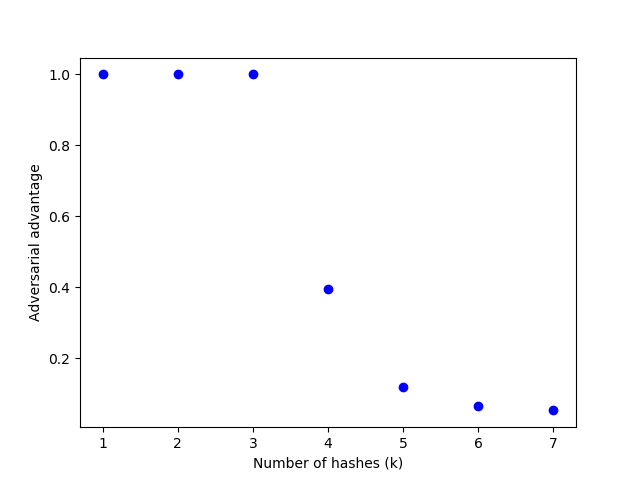
\includegraphics[scale=0.5]{Figure_1}
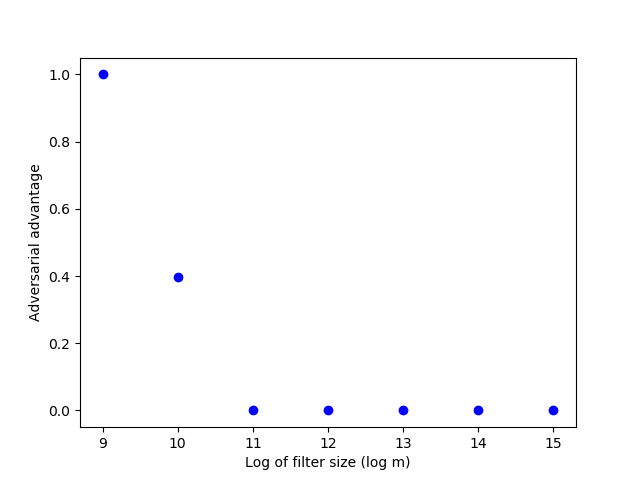
\includegraphics[scale=0.5]{Figure_2}
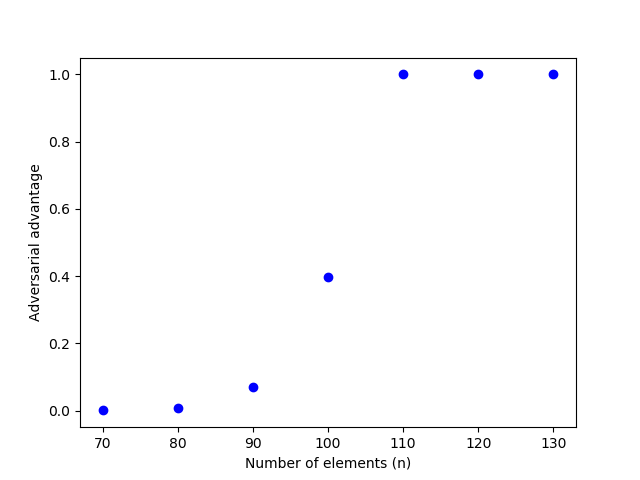
\includegraphics[scale=0.5]{Figure_3}
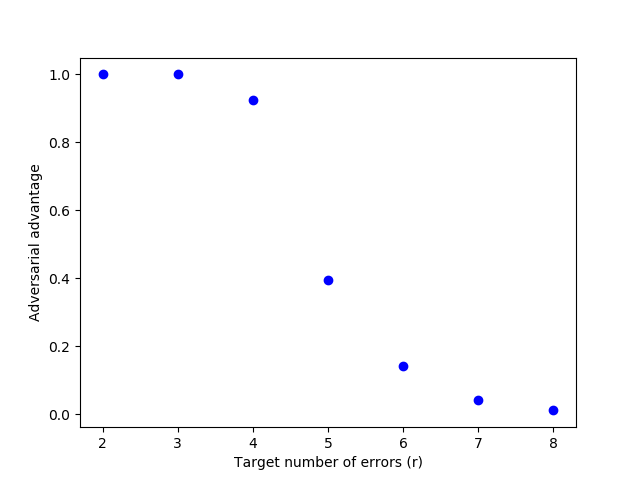
\includegraphics[scale=0.5]{Figure_4}
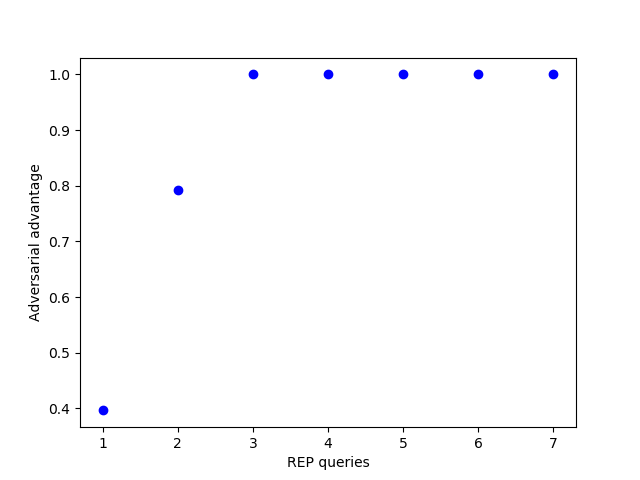
\includegraphics[scale=0.5]{Figure_5}
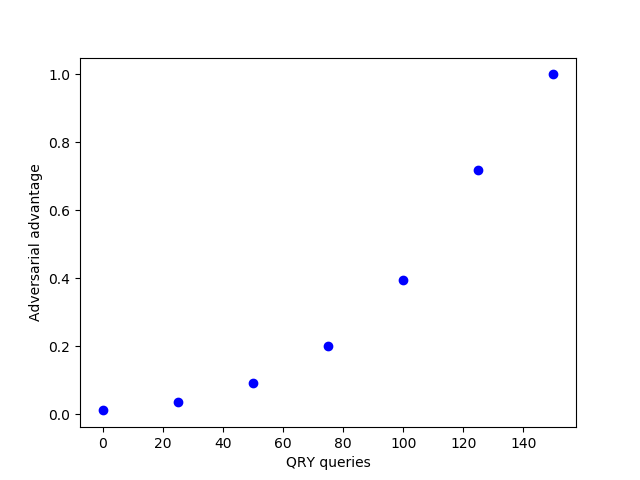
\includegraphics[scale=0.5]{Figure_6}
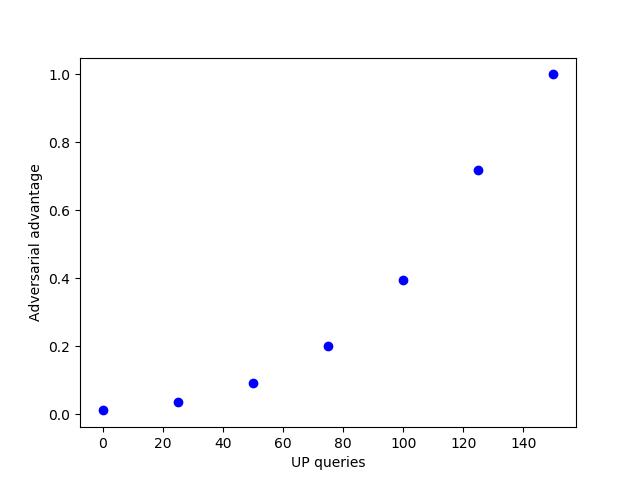
\includegraphics[scale=0.5]{Figure_7}

\subsection{Counting filter results}

Next, we consider the case of a counting Bloom filter. In this setting, an update to add an element increments each of the counters mapped to by the hash functions, with some maximum ceiling $c$ above which the counter cannot increase. A Bloom filter would then just be a counting Bloom filter with a maximum counter value of 1, but we make the additional change that a counting Bloom filter can perform delete operations which work by hashing the element and decrementing the counters at those indices.

Because a counting filter without deletion behaves identically (in terms of responding to queries) to a standard Bloom filter, any attack on a Bloom filter can be trivially converted into an attack against a counting filter simply by performing the exact same operations in the same order. This means that the adversarial advantage against a counting filter, under any of the correctness notions and using any parameters, is bounded below by the advantage against a Bloom filter with the same parameters.

This lower bound is not tight, however, since there are some attacks which exploit the more powerful $\UPO$ oracle provided to the adversary in the case of a counting filter. Consider the public-representation case for an example, where we suppose the structure makes use of a per-representation salt. With a counting filter, the adversary is able to construct representations of arbitrary singleton sets using a single $\REPO$ call and multiple $\UPO$ calls. They begin the game by using $\REPO$ to initialize an empty filter. Then, for some each element $x_1, \ldots, x_{|\col|}$ that the adversary wishes to test, they may first use $\UPO$ to insert the element and then use a second $\UPO$ call to delete the element, returning again to an empty filter. After determining the representation of each singleton subset of $\col$, they can again find $\setT$, $\setR \subseteq \col$ offline computations, where each element of $\setR$ is a false positive for the representation of $\setT$. Since there is only a single representation being manipulated, the salt is in fact constant across the entire experiment. This attack requires a single $\REPO$ call to initialize the filter, $2|\col|$ calls to $\UPO$ to test the elements plus an additional $|\setT|$ calls to $\UPO$ to reinsert the elements found to produce false positives, and $|\setR|$ calls to $\QRYO$ to win the experiment.

In order to achieve good security for a counting filter, it is necessary to use the thresholding assumption that insertions are rejected when the proportion of nonzero counters in the filter reaches some limit $p$. Without this assumption, the adversary can attempt to optimize the number of nonzero counters while keeping the size of the filter (in terms of the number of elements stored in the underlying set) below some constant maximum value. For example, if some $x$ is known to be a false positive for two different sets $\col_1$ and $\col_2$, this increases the probability that elements of $\col_1$ are false positives for the filter representation of $\col_2$ and vice versa. However, using the assumption that there is a limit on the allowed number of nonzero counters, we can derive a false positive bound similar to that of a standard Bloom filter.

\begin{theorem}[Correctness Bound for Counting Filters]\label{thm:count-bf-bound}
Fix integers $k, m, n, \lambda, r\geq 0$, a threshold ratio $p \in [0,1]$, and an error function $d$.
  For every $t, q_R, q_T \geq 0$, it holds that
  \begin{eqnarray*}
    \Adv{\erreps}_{\struct_\saltybloom,r}(t,&q_R,& q_T, q_U, q_H) \leq \\ && q_R \cdot \left[\frac{q_H}{2^\lambda} + \binom{q_T}{\mu}\left(p+\frac{k\mu}{m}\right]^{k\mu}\right) \,,
\end{eqnarray*}
where $\mu = \lceil r/\max(k \cdot d(0,1), d(1,0)) \rceil$
\end{theorem}

\begin{figure}
  \boxThmBFSaltCorrect{0.48}
  {
    \underline{$\G_0(\advA)$}\\[2pt]
      $\col \getsr \advA^H$; $\setC \gets \emptyset$; $\setB \gets \col$; $\err \gets 0$\\
      $\pub \getsr \Rep[\HASHO](\col)$\\
      $\bot \getsr \advA^{\HASHO,\QRYO,\UPO,\INTO}$\\
      return $(\err \geq r)$
    \\[6pt]
    \oraclev{$\QRYO(x)$}\\[2pt]
      $\setB \gets \setB \cup x$\\
      if $x \in \mathcal{C}$ then return $\bot$\\
      $\setC \gets \setC \union \{x\}$\\
      $a \gets \Qry[\HASHO](\pub, x)$\\
      if $a \neq [x \in \col]$ then $\err \gets \err + 1$\\
      return~$a$
    \\[6pt]
    \oraclev{$\UPO(x,b)$}\\[2pt]
      $\setB \gets \setB \cup x$\\
      $\setC \gets \emptyset$\\
      $a \gets \Qry[\HASHO](\pub, \qry_x)$\\
      if $x \in \setC$ and $b = a \neq [x \in \col]$ then\\
      \tab $\err \gets \err-1$\\
      if $b = 1$ then\\
      \tab $\col \gets \col + \{x\}$\\
      else\\
      \tab $\col \gets \col - \{x\}$\\
      $\pub \gets \Up[\HASHO](\pub,\up_{x,b})$\\
      return~$\bot$
    \\[6pt]
    \oraclev{$\HASHO(x)$}\\
      $\hh \getsr [m]^2$; $\vv \gets \fff(\hh$)\\
      if $T[x]$ is defined then $\vv \gets T[x]$\\
      $T[x] \gets \vv$;
      return $\vv$
  }
  {
    \underline{$\G_1(\advA)$}\\[2pt]
    \oraclev{$\INTO(x,y)$}\\
      if $x \not\in \col$ or $y \not\in \col$ then\\
      \tab return $\bot$\\
      $i \gets 0$\\
      for $h$ in $\HASHO(x)$ do\\
      \tab if $h$ in $\HASHO(y)$ then $i \gets i+1$\\
      return $i$
    \\[6pt]
    \underline{$\G_2(\advA)$}\\[2pt]
    \oraclev{$\UPO(x)$}\\
      if $\QRYO(x)$ and $x \not\in \col$ then\\
      \tab $\err \gets \err + \max(k \cdot d(0,1), d(1,0))$\\
      $\setB \gets \setB \cup x$\\
      $\setC \gets \emptyset$\\
      $a \gets \Qry[H](\pub, \qry_x)$\\
      if $x \in \setC$ and $a \neq [x \in \col]$ then\\
      \tab $\err \gets \err-1$\\
      $\col \gets \col + \{x\}$\\
      $\pub \gets \Up[H](\pub,\up_{x,b})$\\
      return~$\bot$
  }
  {
  }
  {
  }
  \caption{Games 0--3 for proof of Theorem~\ref{thm:count-bf-bound}.}
  \label{fig:count-bf-bound}
\end{figure}

\begin{proof}
Applying lemma~\ref{lemma:errep} and lemma~\ref{lemma:salttorand}, we reduce the $\erreps$ experiment to the $\erreps1$ experiment with a salted hash function replaced by true random sampling from $[m]$ for each of the $k$ distinct hash values. This is given in $\G_0$. In $\G_1$, we account for the possibility that the adversary can glean information about the overlap between sets by querying each of them separately. In particular, we give the adversary an additional oracle $\INTO$ that returns the number of locations in which two elements overlap. However, we constrain $\INTO$ to only return an answer when the element has previously been sent to some other oracle.

Because new $\QRYO$ and $\UPO$ calls are based on random sampling, this does not provide the adversary with any additional information about how additional elements which might be queried, inserted, or deleted in the future might behave. However, any element which is sent to $\QRYO$ or $\UPO$ which acts as a false positive will be immediately recognized as such. Because of this, our next step will be to move to a game $\G_2$ where any insertion of a false positive immediately gives the adversary credit for the worst possible error that could be caused by either inserting or deleting that element.

Define $\delta = \max(k \cdot d(0,1), d(1,0))$ and $\mu = \lceil r/\delta \rceil$. In $\G_2$, we modify the game so that producing a false positive increments $\err$ by $\delta$, but so that elements cannot be removed from the set. Because false negatives can only be produced by deleting false positives, and the deletion of $n$ false positives can only produce as many as $nk$ false negatives, this means that the adversary has no need to cause false negatives. Doing so can only decrease the chances of producing additional errors by reducing the values of counters in the filter, and so this does not decerase the adversary's ability to produce errors. Furthermore, we increase the allowed number of nonzero counters from $mp$ to $mp + k\lceil r/\delta \rceil$. The only way in which not being able to remove false positives can decrease the adversary's effectiveness is if the maximum capacity of the filter is reached. Since each false positive removed causes $k$ nonzero counters to be returned to zero, and the adversary stops after accumulating $r$ errors, an allowance of an extra $k\lceil r/\delta \rceil$ nonzero counters is enough to make up for this.

Since each new element queried from outside $\col$ has its corresponding indices determined by a true random function, the adversary can do no better than maximizing the number of nonzero counters in its attempt to produce false positives. Assuming the adversary is able to achieve a maximum-capacity number of nonzero counters, the probability of any particular counter being nonzero is $(mp + k\lceil r/\delta \rceil)/m = p + \frac{k}{m}\lceil\frac{r}{\delta}\rceil$. Over $k$ total hashes, the probability of a false positive is $\left((mp + k\lceil r/\delta \rceil)/m = p + \frac{k}{m}\lceil\frac{r}{\delta}\rceil\right)^k$. Since the adversary needs to accumulate $\lceil\frac{r}{\delta}\rceil$ errors over the course of $q_T$ queries, the probability of the adversary succeeding in this game is

$$\Prob{\G_2(\advA) = 1} = \binom{q_U + q_T}{\mu}\left(p+\frac{k\mu}{m}\right)^{k\mu}$$

Therefore the advantage of the adversary in the original game is

$$\Adv{\erreps}_{\struct_s,r}(\advA) \le q_R \cdot \left(\frac{q_H}{2^\lambda} + \binom{q_T}{\mu}\left(p+\frac{k\mu}{m}\right)^{k\mu}\right).$$\missingqed

\end{proof}

For concrete error bounds, we assume that $d(0,1) = d(1,0) = 1$, so that $\mu = \lceil r/k \rceil$.

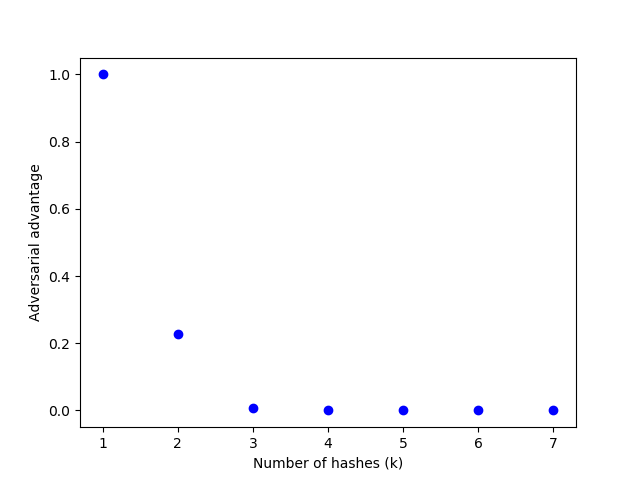
\includegraphics[scale=0.5]{Ct_Figure_1}
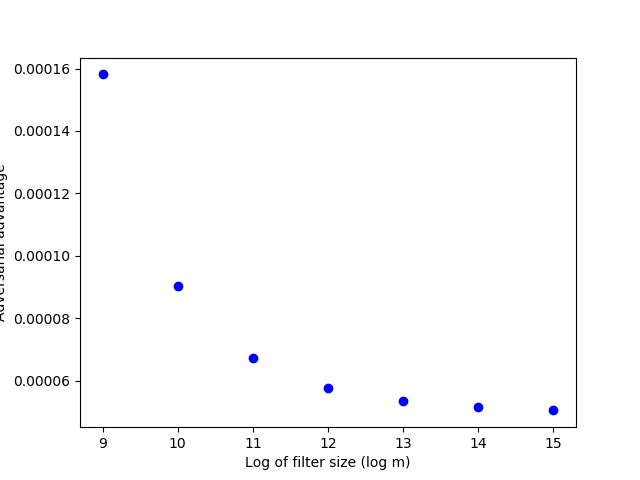
\includegraphics[scale=0.5]{Ct_Figure_2}
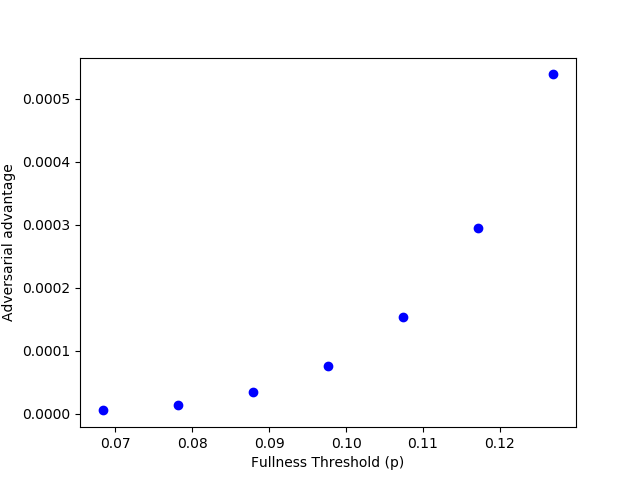
\includegraphics[scale=0.5]{Ct_Figure_3}
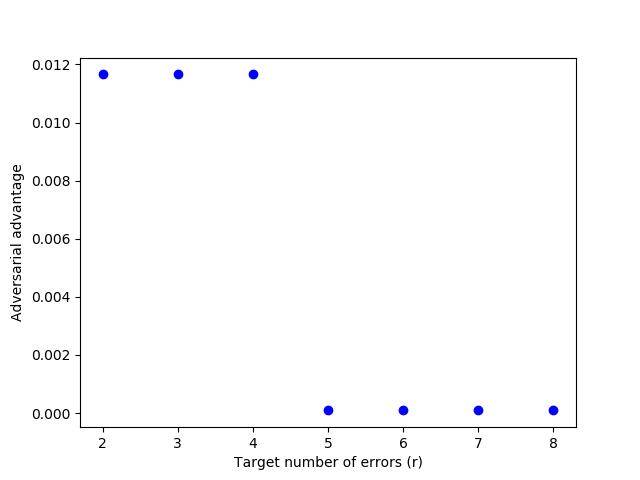
\includegraphics[scale=0.5]{Ct_Figure_4}
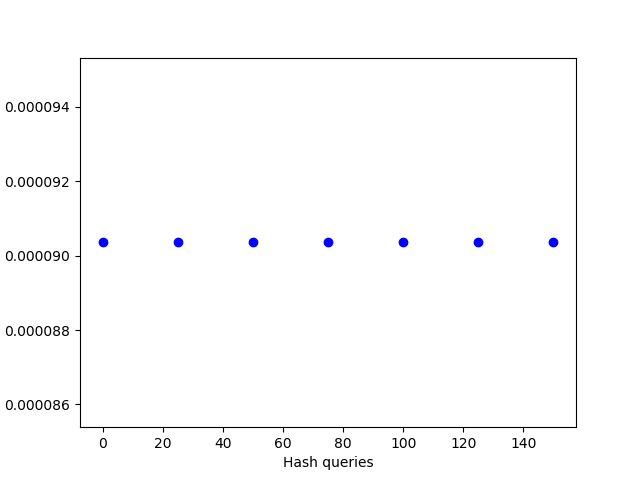
\includegraphics[scale=0.5]{Ct_Figure_5}
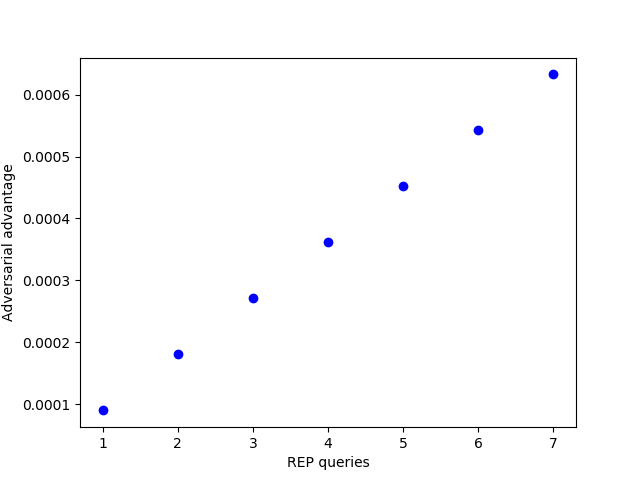
\includegraphics[scale=0.5]{Ct_Figure_6}
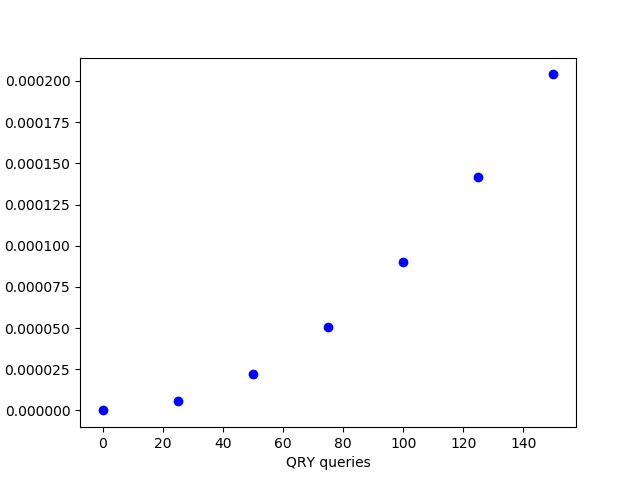
\includegraphics[scale=0.5]{Ct_Figure_7}

%\subsection{Attack on Counting Filters}

%First, $\advA$ chooses an arbitrary set $\col$ of size $n$ and calls $\REPO$ to get a representation of $\col$. The adversary then chooses $q_U$ distinct elements not in $\col$ and makes a series of $\UPO$ calls to remove each of these from the set. Finally, the adversary chooses up to $q_T$ elements from $\col$ and makes a series of $\QRYO$ calls to test for membership of these elements in the set.

%\begin{tabular}{|l|} 
% \hline
% \underline{adversary $\advA$:}\\
% $\col \gets [n]$\\
% $\REPO(\col)$\\
% for $i \in [q_U]$ do\\
% \tab $\UPO(0,\up_{i+n}')$\\
% for $j \in [q_T]$ do\\
% \tab $\QRYO(0,\qry_{j})$\\
% return 0\\
% \hline
%\end{tabular}

\subsection{Cuckoo Filters}

Cuckoo filters provide a way of filtering elements with lower space overhead than counting filters while still allowing for deletion. While they are not as closely related to Bloom filters as counting filters are, and so we do not have the precise lower bound that \textit{any} attack against a Bloom filter also works against a cuckoo filter, it is true that since cuckoo filters are set-membership structures the specific bounds given in the Bloom filter section apply here. To establish acceptable upper bounds, we consider the case of a salted cuckoo filter with private representations. By `salted', we mean that both the hashing and the fingerprinting makes use of a salt chosen on a per-represntation basis. Using this definition, we can make use of the lemmas that allow us to talk about the structure in the single-represntation case with true random functions. A bound for the false positive rate in cuckoo filters is given by $\binom{n}{2k+1}\left(\frac{2}{2^f \cdot cn}\right)^{2k}$ for a set of $n$ elements in a filter with $b$ entries per bucket and fingerprint size $f$.

\begin{theorem}[Correctness Bound for Cuckoo Filters]\label{thm:cuckoo-salt-bound}
Fix integers $b, k, \lambda, r\geq 0$, where $m \geq \lambda$.
  For every $t, q_R, q_T \geq 0$ such that $q_T \geq r$, it holds that
  $$\Adv{\erreps}_{\struct,r}(t, q_R, q_T, q_U, q_H) \leq q_R \cdot
     \left[
      \frac{q_H}{2^\lambda} +
      {\dbinom{q_T+q_U}{r}} P(b,k+r)^r
    \right]$$
where $P(b,k)$ is the standard, non-adaptive false-positive probability on a cuckoo filter with $b$ buckets of size $k$.
\end{theorem}

\begin{figure}
  \boxThmBFSaltCorrect{0.48}
  {
    \underline{$\G_0(\advA)$}\\[2pt]
      $\col \getsr \advA^H$; $\setC \gets \emptyset$; $\err \gets 0$\\
      $\pub \getsr \Rep[\HASHO](\col)$\\
      $\bot \getsr \advA^{\HASHO,\QRYO,\UPO}$\\
      return $(\err \geq r)$
    \\[6pt]
    \oraclev{$\QRYO(x)$}\\[2pt]
      if $x \in \setC$ then return $\bot$\\
      $\setC \gets \setC \union \{x\}$\\
      $a \gets \Qry[\HASHO](\pub, \qry_x)$\\
      if $a \neq [x \in \col]$ then $\err \gets \err + 1$\\
      return~$a$
    \\[6pt]
    \oraclev{$\UPO(x,b)$}\\[2pt]
      $\setC \gets \emptyset$\\
      $a \gets \Qry[\HASHO](\pub, \qry_x)$\\
      if $x \in \setC$ and $a \neq [x \in \col]$ then\\
      \tab $\err \gets \err-1$\\
      if $b = 1$ then\\
      \tab $\col \gets \col \cup \{x\}$\\
      else\\
      \tab $\col \gets \col \setminus \{x\}$\\
      $\pub \gets \Up[\HASHO](\pub,\up_{x,b})$\\
      return~$\bot$
    \\[6pt]
    \oraclev{$\HASHO(x)$}\\
      $\hh \getsr [m]^2$; $\vv \gets \fff(\hh$)\\
      if $T[x]$ is defined then $\vv \gets T[x]$\\
      $T[x] \gets \vv$;
      return $\vv$
  }
  {
    \underline{$\G_1(\advA)$}\\[2pt]
    \oraclev{$\QRYO(x)$}\\[2pt]
      $\setC \gets \emptyset$\\
      $a \gets \Qry[\HASHO](\pub, \qry_x)$\\
      if $a \neq [x \in \col]$ then\\
      \tab $\err \gets \err+d(a,[x \in \col])$\\
      if $b = 1$ then\\
      \tab $\col \gets \col \cup \{x\}$\\
      else\\
      \tab $\col \gets \col \setminus \{x\}$\\
      $\pub \gets \Up[\HASHO](\pub,\up_{x,b})$\\
      return~$\bot$
    \\[6pt]
    \oraclev{$\UPO(x,b)$}\\[2pt]
      $\setC \gets \emptyset$\\
      $a \gets \Qry[\HASHO](\pub, \qry_x)$\\
      if $a \neq [x \in \col]$ then\\
      \tab $\err \gets \err+d(a,[x \in \col])$\\
      if $b = 1$ then\\
      \tab $\col \gets \col \cup \{x\}$\\
      else\\
      \tab $\col \gets \col \setminus \{x\}$\\
      $\pub \gets \Up[\HASHO](\pub,\up_{x,b})$\\
      return~$\bot$
  }
  {
  }
  {
  }
  \caption{Games 0--3 for proof of Theorem~\ref{thm:cuckoo-salt-bound}.}
  \label{fig:cuckoo-salt-bound}
\end{figure}

\begin{proof}
Again we can use lemma~\ref{lemma:errep} and lemma~\ref{lemma:salttorand} to reduce to the case of $\erreps1$ with true random functions in place of salted hash functions. We use this as the first game $\G_0$, so that $\Adv{\erreps}_{\struct_s,r}(\advA) \le q_R \cdot \left(\frac{q_H}{2^\lambda} + \Prob{\G_0(\advA) = 1}\right).$.

Because membership tests rely on objects having the same fingerprint, and a single bucket may contain multiple copies of the same fingerprint, deleting $n$ false positives can only produce up to $n$ false negatives, one per fingerprint removed. Unless the filter becomes full, it is therefore never helpful for an adversary to delete a false positive, since it cannot increase the number of errors. We may then assume, subject to the condition that the adversary never has to worry about the filter becoming full, that the adversary only makes insertion updates. Furthermore, we may assume the adversary never inserts elements which are already in the set, or elements which have already been queried and found to be false positives, since these also cannot increase the number of errors.

We want to show that alternating between sequences of queries and updates is no better than making updates first and queries afterwards. We have shown that the adversary only makes two types of updates: inserting unqueried elements which are not in the set and inserting known true negatives.

We move to a second game where each $\QRYO$ call also inserts that element. Additionally, the penalty for adding known false positives is removed. To avoid penalizing the adversary by producing an overly-full filter which rejects further insertions, we also increase the size of each bucket by $r$. Because we may assume without loss of generality that the adversary stops after finding $r$ errors, only $r$ false positives will be inserted and so these extra $r$ slots in each bucket are sufficient to ensure that if the buckets in the original game did not fill then the buckets in this game will not fill. Furthermore, we modify $\UPO$ to query for the element before inserting it. This cannot produce a worse result for the adversary, and so $\Prob{\G_0(A) = 1} \le \Prob{\G_1(A) = 1}$. Since $\QRYO$ and $\UPO$ calls are identical and each call is independent of all previous calls, the adversary's probability of success is exactly the probability of accumulating $r$ random errors from queries. Each query is a standard random query to a cuckoo filter, so by the binomial theorem we can get a bound of $\binom{q_T+q_U}{r}P(b,k+r)^r$. This gives the result:

$$\Adv{\erreps}_{\struct_s,r}(\advA) \le q_R \cdot \left(\frac{q_H}{2^\lambda} + \binom{q_U+q_T}{r}P(b,k+r)^r\right).$$\missingqed

\end{proof}

\subsection{Count-Min Sketch}

%The fact that queries can test not just for set membership, but for frequency, means that new attacks are possible. For example, an adversary can pick a set $\col$ and an element $x \not\in \col$ and use $\REPO$ to create several different sketches representing $\col$. If the $\QRYO$ oracle reveals that $x$ is a false positive (i.e. appears in the filter with nonzero frequency) for any of these, the adversary can use $\UPO$ to insert all the elements of $\col$ an additional $r$ times. Then a single further $\QRYO(x)$ call will produce an error of magnitude $r$, causing the adversary to succeed at the experiment.

%The success rate of this attack depends on $|\col|$. The probability of $x$ being a false positive is given by the standard Bloom filter bound, $(1-e^{-k|\col|/m})^k$ for a $k$-by-$m$ count-min sketch. Since the adversary needs $(r-1)|\col|$ calls to $\UPO$ to produce an error of size $r$

The fact that queries can test not just for set membership, but for frequency, means that new attacks are possible. For example, the adversary can pick a set $\col$ and an element $x \not\in \col$. They then use $\REPO$ to create several different sketches representing a multiset containing each element of $\col$ exactly $c$ times, where $c$ is the smallest natural number such that $d(c,0) \ge r$, and uses $\QRYO$ to test $x$'s membership in each of these. A single such mistake is by definition sufficient for the adversary to win the experiment, so the probability of adversarial victory is the same as the probability of an adversary finding a single element that creates a hash collision in each of the $k$ rows of the sketch. Winning at the $r$-error game with a set of size $n$ can therefore be reduced to the problem of winning at the $r'$-error game with a set of size $\lfloor\frac{n}{c}\rfloor$, for any $r' > 0$.

% The initial representation, together with n calls to q_U, lets you view n objects; each additional 2n calls to q_U let you view an additional n objects; let the adversary win if they find a single error
% $1-\left(1-\left(1-e^{-n/m}\right)^k\right)^{q_U/(2n)}$

As in the case of counting filters, we are forced to make use of a thresholding assumption, namely that the sum of the absolute values of the counters in the sketch must remain below some upper bound $N$.

%

Depending on the choice of $d$, it is possible no such $c$ exists. One natural choice of $d$ is the Euclidean metric, with $d(x,y) = |x-y|$, but an alternative is to simply define $d(x,y)$ to be 1 if $|x-y| \ge n\epsilon$ and 0 otherwise, where $n$ is the maximum allowed stream size and $\epsilon$ is one of the error parameters. The non-adaptive guarantee for count-min sketch is that each point query has probability no more than $1-\delta$ of producing an error.

What if the threshold for an error is 1? In other words, the adversary gets a point for every `false positive'. Assuming the hash functions are independent, the false positive probability in a count-min sketch is the same as the probability of getting simultaneous false positives in each of $k$ Bloom filters using a single hash function each, which is $\left(1-e^{-n/m}\right)^k$.

%

Given that there is a binary error threshold, we can assume without loss of generality that the adversary never adds an element multiple times, since doing so cannot cause additional errors.

% the adversary can: query for a previously-tested element, query for an untested element, insert an unknown element, insert a known correct element, insert a known overestimated element, insert a known underestimated element, delete an unknown element, delete a known correct element, delete a known overestimated element, or delete a known underestimated element

% inserting an unknown element can increase the number of overestimated elements, and can increase the amount they are overestimated by; it can also decrease the number of underestimaged elements, and can decrease the amount they are underestimated by; it does not affect the estimate of the inserted element
% inserting a known correct element does the same thing, and also does not affect the estimate of the inserted element, so this is equivalent to inserting an unknown element

% inserting any element can increase the number of overestimated elements, and can increase the amount they are overestimated by; it can also decrease the number of underestimaged elements, and can decrease the amount they are underestimated by; it does not affect the estimate of the inserted element; the estimate of the element itself remains unchanged
% the opposite is true for deletion
% there is no upper bound on the number of errors that can be caused by a single insertion or deletion(!)
% in particular, deleting an element immediately causes all otherwise-correct elements that overlap at any point to become off by 1 (too low)

% provide the same $\INTO$ as for a counting filter

%Getting rid of the $q_R$ bound in the salted private-representation case...

%We need a salt, since otherwise the adversary can ask for two representations and reveal one to see what the other looks like.

%In fact, we need independent random representations. Once we have this, seeing representations does not help the adversary. What benefit can there be, then? Suppose an adversary wants to select for representations with certain properties, and ignore others. Since the representation is private, these properties can only be determined by $\QRYO$ calls.